\documentclass[12pt]{report}

\usepackage{graphicx}
\usepackage{enumerate}
\usepackage{listings}
\usepackage[titletoc]{appendix}

\usepackage{url}
\usepackage[bibstyle=ieee]{biblatex}
\setcounter{tocdepth}{3}

\lstMakeShortInline|
%\linespread{1.6}

\makeatletter
\def\@makechapterhead#1{%
  \vspace*{50\p@}%
  {\parindent \z@ \raggedright \normalfont
    %\ifnum \c@secnumdepth >\m@ne
    %    \huge\bfseries \@chapapp\space \thechapter
    %    \par\nobreak
    %    \vskip 20\p@
    %\fi
    \interlinepenalty\@M
    \Huge \bfseries #1\par\nobreak
    \vskip 40\p@
  }}
  \makeatother

\bibliography{final-report}

\title{Bus Tracker: Final Report}

\newcommand{\lstBash}{\lstinline[language=bash,breaklines=true]}

\author{Ian Will, Jason Cluck}
\date{}

\begin{document}
\maketitle

\tableofcontents
\listoffigures

\chapter{Introduction and Motivation}

  Public transportation in the District of Columbia is critical to many of its residents and employees.  The District's public transporation is managed by the Washington Metro Area Transit Authority (WMATA).  WMATA maintains a system of rail and buses that serve most location in the district.  The WMATA rail system is simpler than the bus network and has many maps that are useful for discovering which rail lines server particular regions.  The bus system serves more locations that rail, but can be significantly more perplexing for a new rider.  There are a large number of routes and no comprehensive map, and buses rarely adhere to posted schedules.

\section{Problem Statement}

The Bus Tracker web application provides an interactive map-based overview of the WMATA bus system.  It uses a web API provided by  WMATA to query current bus locations, predictions of arrival times at stops, and full listings of route and stop locations.  This information is then displayed in a clear and interactive manner that displays high-level overviews with easy drill-down for pertinent details (as encouraged by Edward Tufte \cite{tufte:2006}).

\chapter{Requirements Analysis}

\section{Use Cases}

The application is intended for use by those considering or planning to travel on the WMATA bus system.  The primary use case is a smart phone user considering how to catch a bus to an intended destination.  Someone in that situation wonders how long they will be waiting for a bus to arrive at the nearest stop.  They may like to consider alternatives to the bus system such as rail, taxi, or alternate bus route depending on how long they will need to wait for a bus.  They may also like to use Google's traffic overlay to estimate how long the bus will be delayed.

The application will help by showing the anticipated time until the next bus arrives, showing where the next arriving bus is going, and showing nearby stops and routes that may be equally suitable for the intended destination.  This person will probably make location information available to the application through their browser.  The web application may use this information to filter routes and buses that are display to improve performance.  It may also use the location to suggest alternate routes with more promptly ariving buses. 

A second use case is someone at their home or desk computer considering when to leave to minimize wait time at a stop without missing a bus.  The concerns in this case will be similar to to the concerns of the smart-phone user, but location data may not be available.  The person may want a reminder when they need to leave in order to catch their bus.
  

\section{Threshold Requirements}
Threshold requirements describe the minimal set of functionality for a usable product.  These are the requirements that we plan to accomplish.
\begin{enumerate}
\item Display a map of the DC metro region in a web browser
\item Display the browser's reported location on the map if current location is available from the browser
\item Display all WMATA bus routes on the map
\item Display the current locations of all WMATA buses on the map
\item Visually indicate bus direction along with bus position displays
\item Display bus routes using different colors to visually differentiate routes
\item Display bus positions using the same color used for its route
\item Update bus position markers with current positions at five second intervals
\item Display bus stop locations on the map
\item Display the following detail information about a bus stop by clicking on the stop marker
\begin{enumerate}
\item Display the anticipated wait time for the next bus for each route that intersects a given stop
\end{enumerate}
\item Display the following detail information about a bus by clicking on the bus marker
\item Display the stop's WMATA id number
\item Display all bus routes that serve the stop
\begin{enumerate}
\item Bus route name (e.g. ``5A'')
\item Bus headsign (e.g. ``DULLES AIRPORT'')
\item Bus direction (e.g. ``WEST'')
\item Positional uncertainty circle around the bus marker
\end{enumerate}
\end{enumerate}


\section{Objective Requirements}
Objective requirements describe functionality that would improve the quality or usefulness of the application, but are not strictly necessary for a useful product.  These are things we would like to accomplish, but are unsure if time will allow.
\begin{enumerate}
\item Draw DC Circulator bus positions and routes (DC Circulator is not part of the WMATA system)
\item Provide filtering to limit the displayed buses and routes
\begin{enumerate}
\item Filter by only showing routes, stops, and buses matching a route name
\item Filter by only showing routes, stops, and buses matching a headsign
\item Filter by only showing routes with stops wihtin some proximity to the device's current location 
\item Filter by only showing routes with stops wihtin some proximity to an arbitrary location
\item Combine filters using boolean logic, for example only showing routes with stops near current location and some arbitrary location
\end{enumerate}
\item Send a text message or email reminder when a bus is some number of minutes away from a stop
\end{enumerate}

\chapter{Design}

The project to create a live map of DC's Washington Metro Area Transit Authority (WMATA) bus system will be built using the Ruby on Rails web framework, the Google Maps API, WMATA's Transparent Data Sets API, and Twitter's Bootstrap CSS API.

The Google Maps API is used to display the background map, route paths, and bus marker overlays.  Figure \ref{fig:designOverview} shows an overview for how these APIs connect to the Rails web server we're building.

\begin{figure}[ht]
  \centerline{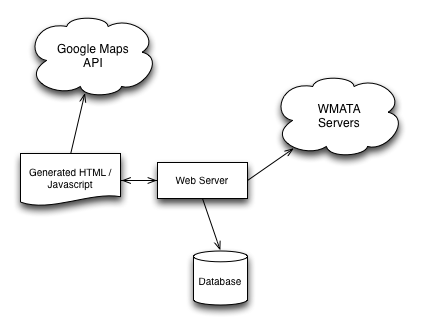
\includegraphics[scale=0.6]{design.png}}
  \caption{API integration overview}
  \label{fig:designOverview}
\end{figure}

The Rails design philosophy favors adopting standard conventions for naming, folder structure, and design patterns across all Rails applications.   This accelerates web development, saving a lot of configuration and rudimentary structuring and naming decision when starting a project.  It also allows the framework to provide numerous helper tools that automate as much as possible.


\section{Model-View-Controller}
The fundamental design pattern adopted by Rails is Model-View-Controller (MVC).  The premise behind MVC is to separate user-interface code (the View), data structures (the Model), and the business logic that connects them (the Controller) into separate modules that can be developed, unit tested, and maintained in isolation.  Figure \ref{fig:MVC} shows the MVC separation as used in the Bus Tracker application.

\begin{figure}[ht]
  \centerline{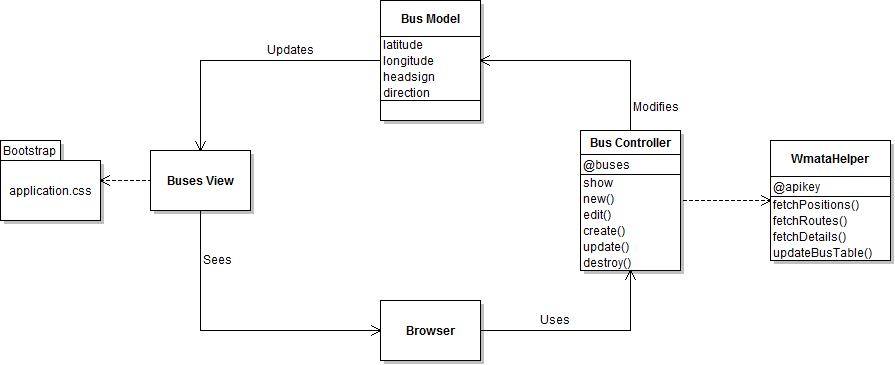
\includegraphics[width=\textwidth]{busTrackerUML.png}}
  \caption{MVC control pattern}
  \label{fig:MVC}
\end{figure}

When an HTTP request comes to the HTTP Server, it first goes to the rails router, which determines which Controller should handle that request.  The controller then uses the Model classes to get the current state of data (e.g. the current position of buses from the database), and passes that information to the View classes.  Rails stores the View logic as HTML with additional preprocessor directives for special scripts called ``partials'' including Embedded Ruby and CoffeeScript.  When these partials are processed by the appropriate preprocessor engine, they have access to variables and data structures provided by the controller.  The preprocessor engine dynamically generates standard HTML and Javascript based on the partial scripts and the data provided by the controller.  These conventions and tools make it easy to prevent business logic from creeping into view code.  They provide a standard idiom for passing data between the model, controller, and view.

Rails adopts the Representational State Transfer (REST) architecture for the HTTP interface.  It uses the inherent HTTP methods (GET, POST, PUT, DELETE) to execute the corresponding Create, Read, Update, Destroy (CRUD) operations on the data model.  This approach is contrasted by the alternative (non-REST) approach of relying predominantly on the HTTP GET method and controlling CRUD behavior using special parameters embedded in the URI \cite{rails}.  Our Bus Tracker application doesn't provide a user-facing capability to create, update, or destroy the model since model updates are fetched from WMATA servers rather than driven by user input.  Therefore the POST, PUT, and DELETE routes have no action associated with them in the controller.  

The GET requests retrieve different types of data depending on the URI requested.  Requesting the root (GET / or GET /index.html) provides the overview map display.  Requesting \lstinline|GET /buses| or GET /buses.json returns the current state of the buses model.  Request GET /stops requests data purely on the stops.  These likely won't be used directly by users, but they are used in the Javascript that asynchronously updates the map display.  Periodically a Javascript request is made to /buses.json to retrieve an updated array of bus positions in the JSON format.  

Some of the API features specific to Bus Tracker are listed in Figure \ref{fig:MVC}.  The controller relies on fetching data from the WMATA servers which  are accessed via a helper class - WmataHelper.  WmataHelper fetches the current position of all buses from the WMATA servers and stores that data in using the model classes. 

 Bus Tracker also uses is Twitter's Bootstrap API which provides additional CSS options. Combining Bootstrap with the View can create dynamic web pages that can render correctly on phones or desktop computers with minimal overhead.

\section{Model Relationships}

Bus Tracker will contain information regarding all the buses served by WMATA.  This includes bus information (including positions), stop information, and route information (including way points describing the route).  Figure \ref{fig:busEntity} shows the entities and relationships between the WMATA data used by Bus Tracker.  This is the information that will be stored locally after retrieving the information from WMATA.

\begin{figure}[ht]
  \centerline{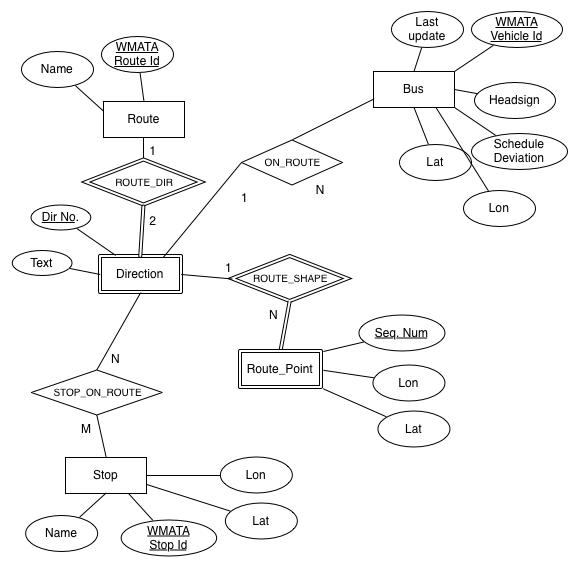
\includegraphics[scale=0.43]{bus-entity-rel.png}}
  \caption{Model relationship diagram}
  \label{fig:busEntity}
\end{figure}

Figure \ref{fig:busSchema} shows the schema that Bus Tracker uses to store information about the current state of the WMATA bus system.  This persists all necessary information on routes, buses, and stops.  Underlined fields indicate primary keys, arrows indicate foreign key dependencies on primary keys from other tables.  

\begin{figure}[ht]
  \centerline{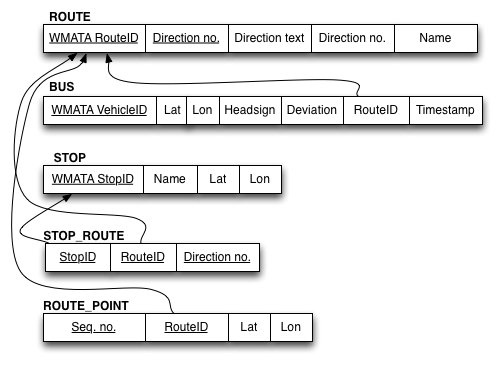
\includegraphics[scale=0.6]{bus-schema.png}}
  \caption{Schema for WMATA API}
  \label{fig:busSchema}
\end{figure}


\chapter{Implementation Details}

Bus Tracker was implemented using the Ruby on Rails web framework, and the Google Maps Javascript API.  The Rails application interfaces with WMATA servers and maintains its own representation of the current state of the WMATA server in its databases.  It polls this periodically and updates its database accordingly.  

The rails server implements a traditional Create / Retrieve / Update / Destroy (CRUD) interface when /routes/, /stops/ and /buses/ are visited.  The main page, however (/) is is a full page map with icons that are updated using asynchronous javascript (AJAX).  The asyncronous javascript calls interface with the Rails server to retrieve system state using Javascript Object Notation (JSON).  These JSON representations are parsed in the client-side javascript and the map icons are updated accordingly.

Information bubbles appear when icons are clicked.  These are populate with HTML that is also generated by the Rails server.  They retrieve HTML from the corresponding REST style url e.g. /buses/1 for the content of the info bubble for a bus with an id of one.  Similarly stop info is populated using /stops/1.  Next bus predictions for a particular stop are retrieved using /stops/1/prediction.  These paths can be entered directly into the browser, and the information will be displayed outside of the map context.



Stops:  11321
Routes: 352
Buses:  648

\section{Bootstrap}

Twitter's Bootstrap API was used to overwrite the default CSS provided by Rails scaffolding.  Bootstrap has recently emerged as a versatile toolbox of html and css classes.  Bootstrap was used in Bus Tracker to include a collapsible navigation bar that allows for the application to be used on browsers with smaller windows such as mobile devices.  The collapsed navbar provides a list of buttons that can be recessed if the user wants to see more of the map, making it ideal for this application.  Other uses include a Modal unit for the About section which provides a nice javascript enabled window which drops down over the UI.  Utilizing Bootstrap did create some problems with Google Maps but this was resolved by customizing the CSS classes.
\cite{bootstrap}
\section{Deployment on Heroku}

Heroku was chosen as the hosting for the production environment due to its easy of deployment with Rails applications and usage with Git.  Although deploying with Heroku was easy at first, there were some things that required work additional work.  The first problem we encountered was how to continually poll for data in the background while not stalling the main application thread.  This was done by using a Heroku Worker in conjunction with the Delayed Job gem.  This gem allows any Active Record object to be added to a priority queue which the Worker handles.  With this solved, there still was the issue of having the code run every 10 seconds (the minimum value before exceeding the threshold).  To fix this, A Heroku Clock Singleton process was added (in the form of an additional Dyno) that kept track of what tasks were ready to be run.  The Clockwork gem combines with the Heroku Clock to specify what tasks the Heroku Clock should run.  An example of a poll would include the Heroku Clock seeing that it needs to run something (as specified by Clockwork), and then adds it to the Delayed Job queue. The Heroku Worker picks up the task from the queue and processes it -- updating all of the bus locations. \cite{heroku}


\chapter{Test Cases}

\section{Test Overview Page}
\begin{enumerate}
\item Run the Rails server \lstBash|rails server|
\item Run the update daemon \lstBash|script/daemon run poll_buses.rb|
\item Load root web page (http://localhost:5000)
\begin{enumerate}
\item Route KML should load, showing bus routes with various colors
\item Bus icons should display after a brief delay
\item At least a few bus icons should be somewhat opaque
\item Bus colors should match route colors
\item After a few minutes, at least a few buses should bounce to indicate new position data
\end{enumerate}
\end{enumerate}

\section{Test Bus Information Window}

\section{Test Route Focus}

\section{Test Stop Information Window}

\section{Test Non-Map Interface}
\begin{enumerate}
\item Run the Rails server \lstBash|rails server|
\item Run the update daemon \lstBash|script/daemon run poll_buses.rb|
\item Load routes page in a browser (http://localhost:3000/routes/)
\item Load stops page in a browser (http://localhost:3000/stops/)
\item Load buses page in a browser (http://localhost:3000/buses/)
\end{enumerate}


\chapter{Task Breakdown and Timeline}
\begin{description}
  \item Tasks to be done by:  November 10, 2012   
  
  \begin{enumerate}
    \item Initial rails setup [Cluck]
    \item CSS styling using twitter bootstrap [Cluck]
    \item Display map on index page [Cluck]
    \item Fetch bus positions from WMATA servers [Will]
    \item Store WMATA response in database [Will]
    \item Draw markers on map for bus locations [Will]
    \item Draw lines on map for bus routes [Will]
    \item Display initial map area based on geo-location reading [Cluck]
    \item Show info window when bus marker is clicked, including the following [Will]
    \begin{enumerate}
      \item Route name
      \item Schedule deviation (lateness)
      \item Time of last position update (data staleness)
      \item Headsign
      \item Direction
    \end{enumerate}
  \end{enumerate}
  \item Tasks to be done by: November 20, 2012
  \begin{enumerate}
    \item Fetch routes from WMATA servers [Will]
    \item Fetch stops from WMATA servers [Will]
    \item Store routes in database [Cluck]
    \item Store stops in database [Cluck]
  \end{enumerate}
  \item Tasks to be done by: December 3, 2012
  \begin{enumerate}
    \item Display bus stops with markers on map [Cluck]
    \item Control WMATA polling to avoid exceeding usage limits [Will]
    \item Show info window when stop marker is clicked [Will]
      \begin{enumerate}
        \item Show which routes and directions the use the stop
        \item Show next bus wait time projections for each route that uses the stop
      \end{enumerate}
    \item Show info window when stop marker is clicked [Will]
    \begin{enumerate}
      \item Retrieve HTML from Rails stops/:id path
      \item Use AJAX to update next bus arrival predictions from WMATA
    \end{enumerate}
    \item Orient bus markers according to direction traveled
  \end{enumerate}
\end{description}

\addcontentsline{toc}{chapter}{References}
\printbibliography

\begin{appendices}
\chapter{User Manual}

The Bus Tracker web application immediately presents an overview of the current state of the WMATA system.  All routes are shown as KML overlays, and current positions of buses on those routes are indicated with bus icons.  This initial state is shown in Figure \ref{fig:busOverview}.

\begin{figure}[ht]
  \centerline{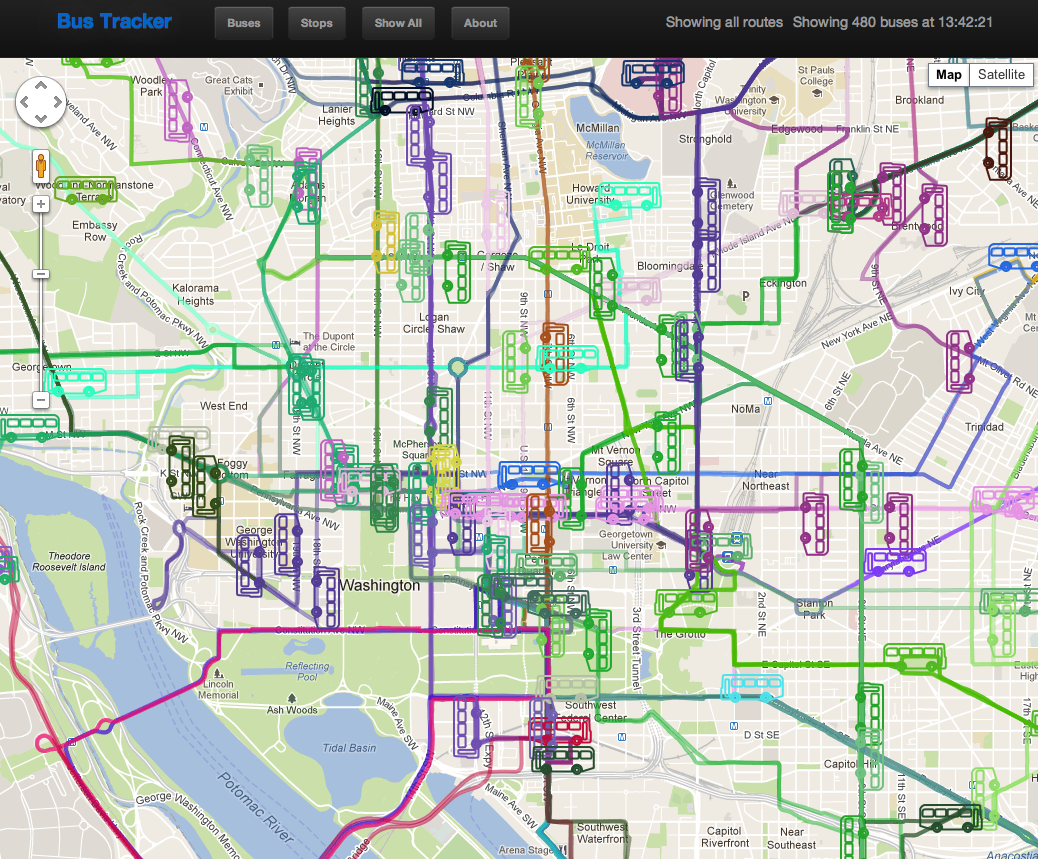
\includegraphics[width=\textwidth]{bus-tracker-overview.png}}
  \caption{Overview of WMATA Bus System}
  \label{fig:busOverview}
\end{figure}


Bus icons move as their position information is updated on WMATA's servers.  These updates do not come from WMATA as frequently as desired, which is a limitation of their system.  Buses typically are updated within a two minute time span, but the delay can sometimes be much longer.  When position updates are received for a bus, its icon bounces a few times to indicate a change in position.  

The age of a bus position can be quickly determined based on the opacity of a bus icon.  A transparent icon has position information that is more than five minutes old.  The more opaque a bus icon is shaded, the more recent its position information.  The exact age of the bus position information can be seen in the bus information window that displays when clicking on a bus icon.  An example is shown in Figure \ref{fig:bus-details}.  It includes route name, direction, headsign, age of position data, vehicle id number, and deviation from the posted schedule.

\begin{figure}[ht]
  \centerline{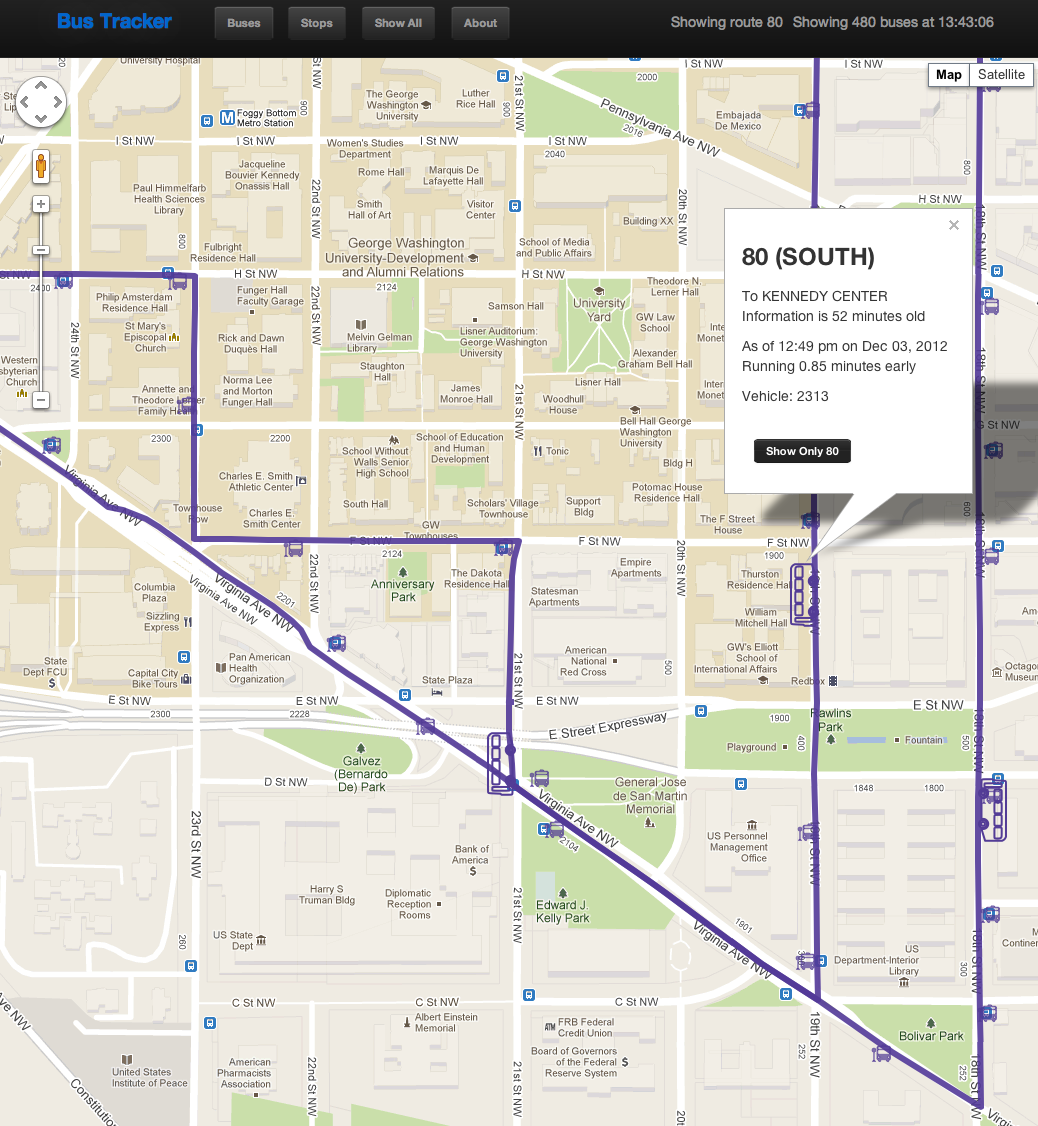
\includegraphics[width=\textwidth]{bus-info-bubble.png}}
  \caption{Bus Detail Window}
  \label{fig:bus-details}
\end{figure}


Initially all buses and all routes are displayed.  This can be a nice overview, but can also be visually overwhelming.  Bus Tracker allows you to focus in on a route, showing only its path, buses, and also displaying the stops thoses buses serve.  There are two ways to focus on a route.  One is by clicking on the route path, then clicking ``Show Only Route D2'' on the tool bar (where D2 is route clicked).  The second way to focus on a specific route is to click the ``Show Only D2'' button in a bus information window.  This will focus on the route that the bus is serving.

When a specific route is in focus, the stops on that route are also shown.  Clicking on a stop icon brings up a stop information window (Figure \ref{fig:stop-details}).  Stop information windows show the stop's name, its WMATA stop ID (which other applications use to look up bus arrival predictions), a table of predicted bus arrival times, all routes that serve this stop, and the stop coordinates.

\begin{figure}[ht]
  \centerline{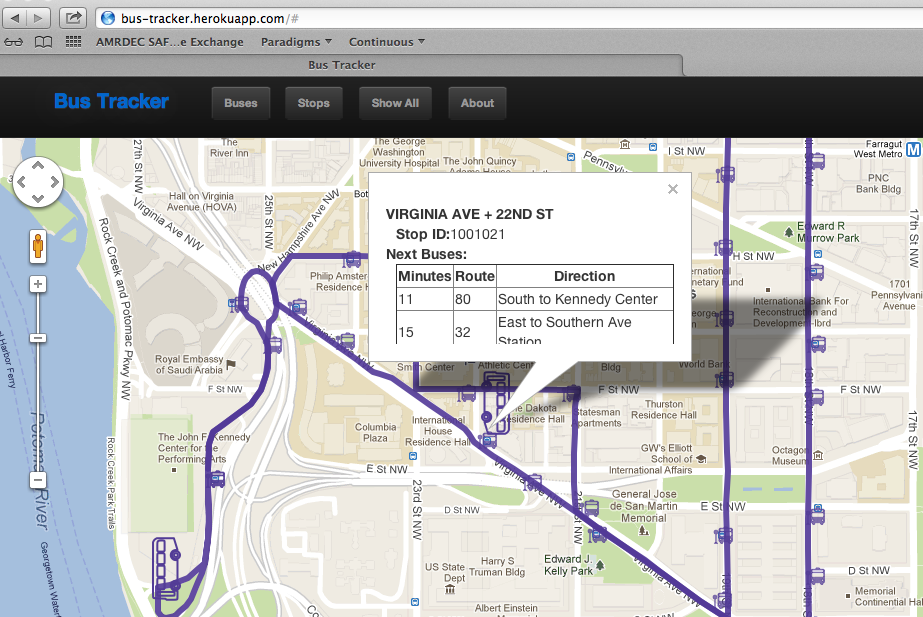
\includegraphics[width=\textwidth]{stop-info-bubble.png}}
  \caption{Stop Detail Window}
  \label{fig:stop-details}
\end{figure}

The bus arrival predictions shown in the stop information window are more accurate than bus position data.  They are provided by WMATA's API, and project bus arrival based on last-known location and average bus speed.

\end{appendices}


\end{document}

